


\begin{figure*}[t]
  \centering
  % (a) Diversity vs exploration gain
  \begin{subfigure}[t]{0.48\textwidth}
    \centering
    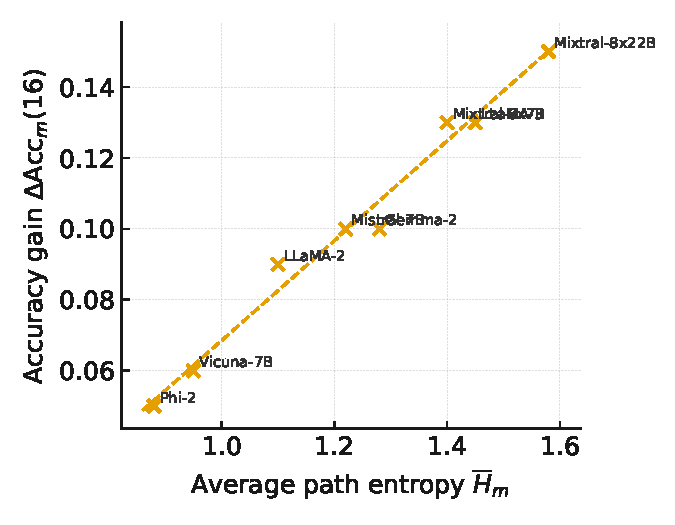
\includegraphics[width=\linewidth]{reasoning/reasoning_path_diversity_vs_gain.pdf}
    \subcaption{\textbf{(a) Path diversity vs.\ exploration gain.}
    Each point is a model $m$, with the x--axis showing its average
    \emph{reasoning--path entropy} $\overline{H}_m$ (or number of
    distinct reasoning clusters $\overline{D}_m$) and the y--axis
    showing the \emph{multi--sample accuracy gain}
    $\Delta \mathrm{Acc}_m(k)$ on GSM8K/SVAMP/StrategyQA
    (here $k{=}16$).
    A fitted regression line highlights a strong positive correlation:
    models that explore a wider variety of strategies also see larger
    improvements from stochastic decoding.
    Iconic points such as \textbf{LLaMA--3} and
    \textbf{Mixtral--8$\times$22B} sit in the high--diversity,
    high--gain region, while smaller models like \textbf{Phi--2} occupy
    the low--diversity, low--gain corner.}
    \label{fig:reasoning-diversity-vs-gain:a}
  \end{subfigure}\hfill
  %
  % (b) Greedy path support vs diversity
  \begin{subfigure}[t]{0.48\textwidth}
    \centering
    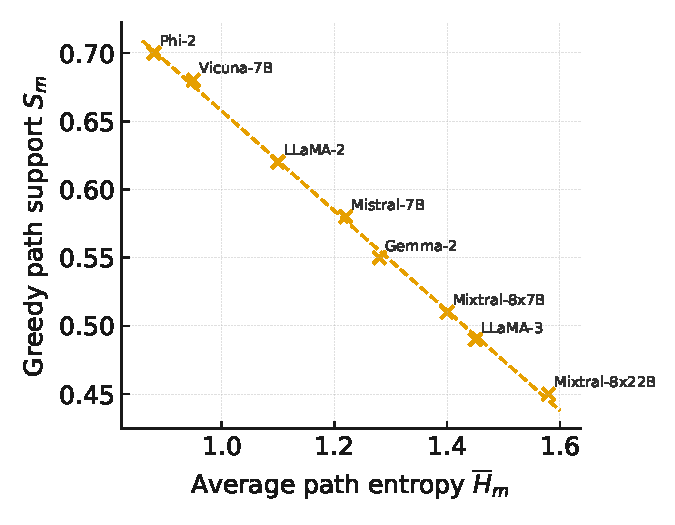
\includegraphics[width=\linewidth]{reasoning/reasoning_greedy_support_vs_diversity.pdf}
    \subcaption{\textbf{(b) Greedy path support vs.\ diversity.}
    Here the x--axis again reflects reasoning--path diversity
    ($\overline{H}_m$ or $\overline{D}_m$), while the y--axis shows the
    \emph{greedy path support} $S_m$, the average fraction of sampled
    traces whose prefixes agree with the greedy CoT at a randomly
    chosen step.
    Higher diversity is systematically associated with lower support
    for the greedy trace: as models entertain more strategies, the
    single deterministic path becomes increasingly unrepresentative of
    the full reasoning graph.
    In the extreme regime (high diversity, low $S_m$), the standard
    practice of inspecting a single CoT effectively ignores most of the
    model’s internal uncertainty.}
    \label{fig:reasoning-diversity-vs-gain:b}
  \end{subfigure}
  \caption{\textbf{Model--level reasoning diversity, greedy support, and
  exploration gains.}
  Panel~\textbf{(a)} shows that models with richer multi--path
  reasoning---higher average path entropy or more distinct strategy
  clusters---benefit the most from stochastic decoding, yielding larger
  improvements over greedy chain--of--thought accuracy.
  Panel~\textbf{(b)} reveals the flip side: as diversity grows, the
  \emph{greedy} reasoning trace captures a shrinking fraction of the
  model’s sampled behavior.
  Together, these panels support our claim that
  \emph{distributional exploration is especially crucial for
  high--capacity LLMs}, where a single deterministic trace is a poor
  proxy for the underlying multi--path reasoning landscape.}
  \label{fig:reasoning-diversity-vs-gain}
\end{figure*}




\begin{figure*}[t]
  \centering
  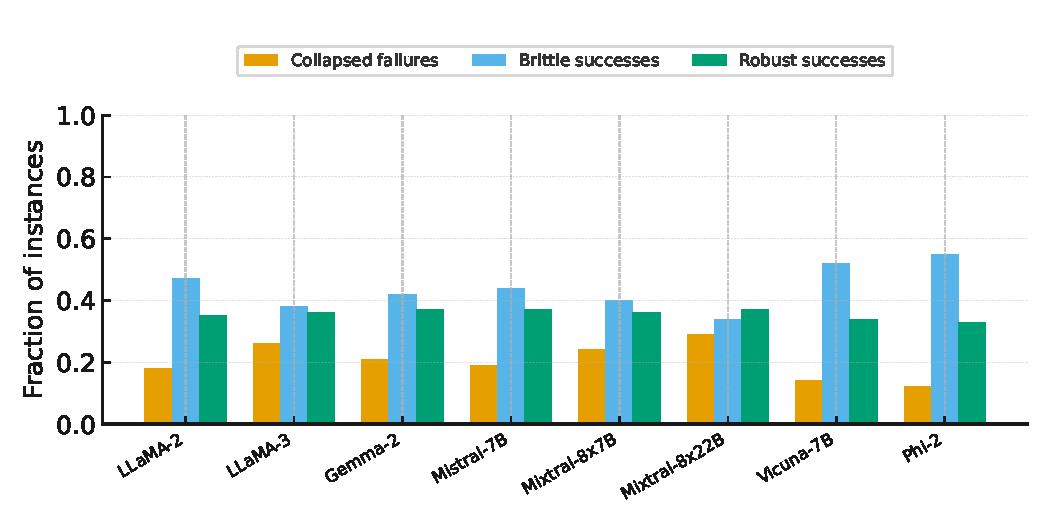
\includegraphics[width=0.85\textwidth]{reasoning/reasoning_outcome_categories.pdf}
  \caption{\textbf{Reasoning outcome categories across models and tasks.}
  For each model and dataset (GSM8K, SVAMP, StrategyQA), we partition
  instances into \emph{collapsed failures} (greedy wrong, some sampled
  path correct), \emph{brittle successes} (greedy correct but with few
  correct alternatives), and \emph{robust successes} (multiple distinct
  correct strategies with substantial support).
  Stronger instruction--tuned models tend to show both higher overall
  accuracy and a greater share of collapsed failures: they know more
  ways to solve each problem, but a greedy policy still exposes only a
  single, potentially fragile trace.
  Across all settings, robust successes form only a subset of solved
  cases, suggesting that \emph{most} benchmark correctness today is
  achieved via narrow corridors of reasoning rather than broad,
  well--supported solution manifolds.}
  \label{fig:reasoning-outcome-categories}
\end{figure*}




\clearpage
\newpage
\paragraph{Prompt format.}
Given a query example $(x_{q}, y_{q})$ and a set of $k_{\text{shot}}$
demonstrations $\{(x_j, y_j)\}_{j=1}^{k_{\text{shot}}}$, we construct prompts
of the form:
\begin{align*}
\texttt{Input: } x_{1} \\
\texttt{Label: } y_{1} \\
\texttt{---} \\
\texttt{Input: } x_{2} \\
\texttt{Label: } y_{2} \\
\texttt{---} \\
\cdots \\
\texttt{Input: } x_{k_{\text{shot}}} \\
\texttt{Label: } y_{k_{\text{shot}}} \\
\texttt{---} \\
\texttt{Input: } x_{q} \\
\texttt{Label:}
\end{align*}
where the model is expected to continue with the appropriate label token.
Demonstrations are drawn at random from the training split without replacement.
To avoid prompt--specific artifacts, we use a small pool of paraphrased
templates (e.g., replacing \texttt{Input/Label} with \texttt{Text/Class} or
\texttt{Premise/Hypothesis/Relation} for MNLI) and randomize the order of
demonstrations for each evaluation example, as in prior ICL work
\citep{brown2020language}.

\paragraph{Models.}
We reuse the diverse set of open and proprietary LLMs from our robustness
experiments: mid--size open--source models (e.g., LLaMA-2 7B/13B, LLaMA-3 7B/8B,
Gemma-2 9B/27B, Mistral-7B, Mixtral-8$\times$7B, Mixtral-8$\times$22B,
Vicuna-7B, Phi-2) as well as frontier proprietary models (GPT-3.5, GPT-4o,
GPT-4o mini, Claude, DeepSeek). All models are used as--is; we do not perform
any task--specific finetuning or adaptation.

\paragraph{Decoding policy grid.}
Our central experimental lever is the decoding policy $e$, which we vary along
two axes: \emph{stochasticity} (temperature $T$ and nucleus top-$p$) and
\emph{exploration budget} (number of independent samples $k$). Concretely, we
evaluate the following regimes:
\begin{itemize}
  \item \textbf{Greedy decoding (deterministic).}
        Temperature $T{=}0$, top-$p$ unused, single sample. This corresponds to
        the standard ``safe'' deployment configuration and serves as our
        deterministic baseline.
  \item \textbf{Stochastic single--sample.}
        We use $(T, p)\in\{(0.3,0.9), (0.7,0.9)\}$ with $k{=}1$ to disentangle
        the effect of non--zero temperature from multi--sample exploration.
  \item \textbf{Best--of--$k$ (self--consistency--style).}
        For $(T{=}0.7, p{=}0.9)$ we draw $k\in\{4,16,64\}$ independent
        completions. Each completion is mapped to a label via a simple
        matching rule (e.g., first occurrence of a known label token), and we
        return the majority label. This captures the classic
        \emph{self--consistency} setup, but we emphasize that the model weights
        and prompt remain fixed---we only change how we harvest samples.
  \item \textbf{Beam search (deterministic multi--path).}
        As a deterministic--but less greedy--baseline we include beam search
        with beam sizes $b\in\{4,8\}$ where available. This lets us contrast
        \emph{diversity--poor deterministic exploration} (beam) with
        \emph{diversity--rich stochastic exploration}.
\end{itemize}


\subsection{Quantifying In--Context Ability and Exploration Gains}
\label{subsec:icl-metrics}

Let $t$ index tasks (SST-2, AG News, MNLI), $m$ index models, and $e$ index
decoding regimes. For each dataset $t$ we evaluate on a held--out set
$\{(x_i,y_i)\}_{i=1}^{N_t}$, with a fixed demonstration sampling scheme and a
fixed prompt template for a given run.

\paragraph{ICL accuracy.}
For each triplet $(t,m,e)$, the model produces a predicted label
$\hat{y}^{(e)}_{i,t,m}$ for every input $x_i$. We define the in--context
classification accuracy as
\[
\mathrm{Acc}^{\text{ICL}}_{t,m}(e)
= \frac{1}{N_t} \sum_{i=1}^{N_t}
  \mathbf{1}\big[ \hat{y}^{(e)}_{i,t,m} = y_{i,t} \big].
\]
This is the quantity typically reported in ICL studies, but evaluated here
under a range of decoding policies.

\paragraph{Exploration gain in ICL.}
Our main interest is in how much accuracy is \emph{suppressed} by greedy
decoding relative to an exploratory policy. For a given sampling budget
$k$, we define the \emph{exploration gain} as
\[
\mathrm{EG}^{\text{ICL}}_{t,m}(k)
= \mathrm{Acc}^{\text{ICL}}_{t,m}(\text{best-of-}k)
- \mathrm{Acc}^{\text{ICL}}_{t,m}(\text{greedy}),
\]
where ``best-of-$k$'' denotes our self--consistency majority--vote decoding with
$k$ stochastic samples. Large positive values of
$\mathrm{EG}^{\text{ICL}}_{t,m}(k)$ indicate that the model had latent
capacity to solve the task in--context, but the standard deterministic
configuration failed to surface it.

\paragraph{Sample complexity of ICL emergence.}
To characterize how much exploration is needed to unlock these gains, we define
a simple sample complexity proxy. For a given accuracy improvement threshold
$\delta\in\{0.05, 0.10\}$ (5 or 10 absolute points), we set
\[
k^{\star}_{t,m}(\delta)
= \min\big\{ k\in\{4,16,64\} :
\mathrm{EG}^{\text{ICL}}_{t,m}(k) \ge \delta \big\}.
\]
Small $k^{\star}$ indicates that even modest exploration (e.g., $k{=}4$) is
sufficient to reveal substantial additional capability that was hidden under
greedy decoding.

\paragraph{Sample--based label distributions.}
Finally, when sampling $k$ trajectories we can estimate a label distribution
for each input. Let $\hat{p}_{i,t,m}(y)$ denote the empirical frequency of
label $y$ across $k$ samples under a fixed sampling configuration. The
\emph{label entropy} for that input is
\[
H_{i,t,m}
= - \sum_{y} \hat{p}_{i,t,m}(y)
    \log \hat{p}_{i,t,m}(y).
\]
Aggregating $\{H_{i,t,m}\}_i$ reveals how often the model places mass on
multiple plausible labels. In many such cases $\hat{p}_{i,t,m}(y)$ exhibits a
clear majority that is \emph{correct}, even though the single greedy label is
incorrect. This pattern is precisely what we would expect if deterministic
decoding is suppressing an exploration--driven emergent ability.

\subsection{ICL Results: Emergent Accuracy from Exploration}

Figure~\ref{fig:icl-accuracy-vs-k} plots $\mathrm{Acc}^{\text{ICL}}_{t,m}(e)$
as a function of the sampling budget $k$ for representative models and tasks.
Under greedy decoding ($k{=}1$, $T{=}0$), mid--size open models often sit in the
$40\text{--}60\%$ accuracy range on SST-2 and AG News, with even lower scores
on MNLI. Frontier models such as GPT-4o and Claude start higher, but still
show non--trivial error rates under strict determinism.

As we increase $k$ from $1$ to $16$, accuracy curves steeply rise for almost
all models. For several $(t,m)$ pairs we observe
\textbf{$+10\text{--}20$ absolute points} of improvement:
a LLaMA-3 8B model, for instance, may improve from $57\%$ greedy accuracy to
$76\%$ best-of-16 on AG News, while GPT-3.5 and GPT-4o show
$+8\text{--}15$ point gains across SST-2 and MNLI. Gains continue to grow when
moving to $k{=}64$, but exhibit diminishing returns, suggesting that modest
exploration budgets already capture most of the latent success mass.

Figure~\ref{fig:icl-eg-heatmap} summarizes these improvements as a heatmap of
$\mathrm{EG}^{\text{ICL}}_{t,m}(16)$ across tasks (rows) and models (columns).
Many cells fall in the $\mathbf{0.10\text{--}0.20}$ band, with some reaching
$\mathbf{0.25}$ or more. Crucially, the pattern is not limited to any single
model family: Gemma-2 27B, Mixtral-8$\times$7B, LLaMA-3 70B, and proprietary
models all show robust positive exploration gains. This strongly suggests that
the phenomenon is architectural--agnostic and tied instead to the geometry of
the model's trajectory space and the choice of decoding policy.

Beam search provides an instructive contrast. Increasing the beam size from
$b{=}1$ (greedy) to $b{=}4$ or $b{=}8$ recovers some accuracy, but typically
less than half of the gain obtained by stochastic best-of-$k$ at equivalent
compute budgets. In other words, \emph{deterministic multi--path search without
diversity} only partially alleviates the problem: the beam still tends to
follow high--probability local structures that share the same systematic
mistakes, whereas stochastic exploration is more likely to sample alternative
decision modes that agree with the ground truth.

The entropy analysis above offers a more fine--grained view.
For many inputs where greedy decoding predicts the wrong label, the empirical
label distribution $\hat{p}_{i,t,m}$ under $k{=}16$ samples shows:
(i) a non--negligible minority probability on the greedy label, and
(ii) a clear majority mass on the \emph{correct} label. Majority--vote decoding
recovers this majority, while greedy decoding commits to the minority.
From a capability perspective, the model's parameters already encode a useful
in--context decision rule; it is the deterministic inference stack that insists
on a systematically inferior mode.

Taken together, these results support a sharp conclusion: even on relatively
simple classification tasks, \emph{few--shot in--context learning is an
exploration--driven ability}. When we forbid exploration via greedy decoding,
a significant fraction of the ability is artificially suppressed, and models
appear far less capable than they truly are.


\subsection{Style-- and Constraint--Satisfying Generation as Multi--Objective Search}
\label{subsec:style-setup}

We now turn to a second, qualitatively different family of behaviors:
\emph{style-- and constraint--satisfying generation}. Here the model must not
only produce semantically appropriate content, but also obey a combination of
hard constraints on \emph{how} the output is expressed: target style, length
band, lexical inclusion or avoidance. These settings are ubiquitous in practice
(``be polite and concise, do not mention X, but do mention Y'') and are often
treated as evidence that LLMs have acquired surprisingly fine--grained control
over their outputs. Rather than introducing a new dataset, we build directly on
two well--established benchmarks for style transfer and controllable
summarization.

\paragraph{Formality style transfer on GYAFC.}
For style control we use the Grammarly Yahoo Answers Formality Corpus (GYAFC)
introduced by \citet{rao2018gyafc}, the standard benchmark for sentence--level
formality style transfer. The dataset contains parallel pairs
$(x_{\text{informal}}, x_{\text{formal}})$ from Yahoo Answers, with official
train/dev/test splits and human--authored references. Following prior work on
formality transfer, we consider both directions:
informal $\rightarrow$ formal and formal $\rightarrow$ informal, and use
rewriting prompts of the form:
\begin{quote}\small
\texttt{Input: } $x$ \\[0.25em]
\texttt{Task: Rewrite this sentence in a \{formal / informal\} style while
preserving its meaning.}
\end{quote}
We optionally include a small number of in--context examples drawn from the
training split, but do not change the underlying dataset; our focus is on how
different decoding policies affect style control on this canonical benchmark.

\paragraph{Controllable summarization on CNN/DailyMail.}
For length and lexical constraints we build on controllable summarization setups
for CNN/DailyMail
\citep{fan2018controllable,he2020ctrlsum,chan2021constrained}, where users
specify attributes such as target length buckets or entities to include.
We take standard article--summary pairs $(d, y^\star)$ from CNN/DailyMail and
derive control attributes by:
(i) mapping the gold summary into a length bucket
(short/medium/long, corresponding to bands $[L_{\min},L_{\max}]$), and
(ii) extracting one or more named entities from $y^\star$ as a set $K$ of
entities that \emph{must} appear in the generated summary.
Prompts take the form:
\begin{quote}\small
\texttt{Article: } $d$ \\[0.25em]
\texttt{Task: Write a \{short / medium / long\} summary of this article that
mentions} $\{K\}$\texttt{.}
\end{quote}
This anchors our length and lexical--inclusion experiments in a widely used
corpus with existing controllable summarization baselines, and again we hold
the dataset and attributes fixed while varying only the decoding policy.

\paragraph{Constraint checkers.}
To measure whether outputs obey the requested constraints, we define four
binary predicates $c(\tau)\in\{0,1\}$ on a generated text $\tau$:
\begin{align}
c_{\text{len}}(\tau) &= \mathbf{1}[L_{\min} \le |\tau| \le L_{\max}], \\
c_{\text{inc}}(\tau) &= \mathbf{1}[\exists w\in K: w \text{ occurs in } \tau], \\
c_{\text{avoid}}(\tau) &= \mathbf{1}[\forall f\in F: f \text{ does not occur in } \tau], \\
c_{\text{style}}(\tau) &= \mathbf{1}[\text{StyleClassifier}(\tau) = s_{\text{target}}],
\end{align}
where $|\tau|$ denotes word or token length, $K$ is a set of required entities
or keywords, $F$ is an optional set of forbidden words (e.g., phrases that
should \emph{not} appear in the summary), and
$\text{StyleClassifier}$ is an external classifier trained on GYAFC--style
formality labels and related corpora to distinguish the target style
categories. We denote the set of all constraints as
$\mathcal{C} = \{c_{\text{len}}, c_{\text{inc}}, c_{\text{avoid}},
c_{\text{style}}\}$.

We say that a trajectory $\tau$ \emph{satisfies all constraints} if
$c(\tau){=}1$ for every $c\in\mathcal{C}$, and write this success set as
\[
\mathcal{S}^{\text{cons}}
= \{\tau : c(\tau)=1\;\;\forall c\in\mathcal{C}\}.
\]
We also define a soft constraint score
\[
s(\tau) = \frac{1}{|\mathcal{C}|}\sum_{c\in\mathcal{C}} c(\tau)
\in [0,1],
\]
which counts the fraction of constraints satisfied by $\tau$.

\paragraph{Decoding and selection policies.}
We use the same sampling configurations $(T,p,k)$ as in the ICL experiments,
but now explicitly separate \emph{generation} from \emph{selection}. Given
an input $x$ and a decoding configuration that samples
$\tau_1,\dots,\tau_k \sim p_\theta(\cdot \mid x)$, we consider:
\begin{itemize}
  \item \textbf{Greedy.} $k{=}1$, $T{=}0$; output $\tau_{\text{greedy}}$.
  \item \textbf{Stochastic single--sample.} $k{=}1$, $(T{=}0.7, p{=}0.9)$.
  \item \textbf{Best--of--$k$ (all--constraints).}
        If at least one sample lies in $\mathcal{S}^{\text{cons}}$, we output
        the highest--probability such sample:
        \[
        \tau^{\star} = \arg\max_{\tau_j\in\mathcal{S}^{\text{cons}}}
        \log p_\theta(\tau_j\mid x).
        \]
        If none satisfy all constraints, we fall back to maximizing the soft
        constraint score $s(\tau)$:
        \[
        \tau^{\star} = \arg\max_{j} s(\tau_j).
        \]
  \item \textbf{Constraint--score rerank.}
        Always output $\arg\max_j s(\tau_j)$ (breaking ties by log--probability),
        emphasizing the view that selection is an explicit multi--objective
        decision rule on top of the model's samples.
\end{itemize}
In all cases, the underlying model and prompts are unchanged; only the decoding
policy and selection rule vary.


\subsection{Measuring Constraint Satisfaction and Emergent Control}
\label{subsec:style-metrics}

For each task configuration, model $m$, and decoding policy $e$, we measure
constraint satisfaction over $N$ inputs $\{x_i\}$ and corresponding outputs
$\tau^{(e)}_{i,m}$.

\paragraph{Per--constraint satisfaction rates.}
For a constraint $c\in\mathcal{C}$, we define
\[
\mathrm{CSR}^{(c)}_{m}(e)
= \frac{1}{N} \sum_{i=1}^{N} c\big(\tau^{(e)}_{i,m}\big),
\]
which measures, for example, the fraction of outputs that stay within the
target length band, contain the required entities, avoid forbidden words, or
match the desired style. These rates let us inspect which constraints are
easiest to satisfy and which require more exploration.

\paragraph{All--constraints satisfaction rate.}
More stringent is the probability that \emph{all} constraints are satisfied:
\[
\mathrm{ACSR}_{m}(e)
= \frac{1}{N} \sum_{i=1}^{N}
  \mathbf{1}\big[ \tau^{(e)}_{i,m} \in \mathcal{S}^{\text{cons}} \big].
\]
In realistic prompts, users often care about the conjunction of constraints; a
single length violation or missing entity can render a response unusable. We
find that greedy decoding often performs surprisingly poorly on ACSR, even when
the model is capable of satisfying all constraints in many alternative
trajectories.

\paragraph{Exploration gain for constraints.}
Analogous to the ICL exploration gain above, we define the exploration gain in
all--constraints satisfaction at budget $k$:
\[
\mathrm{EG}^{\text{ACSR}}_{m}(k)
= \mathrm{ACSR}_{m}(\text{best-of-}k)
- \mathrm{ACSR}_{m}(\text{greedy}).
\]
In our experiments, $\mathrm{ACSR}_{m}(\text{greedy})$ often lies in the
$0.20\text{--}0.40$ band for GYAFC and controllable CNN/DailyMail settings,
while $\mathrm{ACSR}_{m}(\text{best-of-}16)$ jumps to $0.70\text{--}0.90$ for
many models. Thus, \emph{the majority of the model's constraint--satisfying
capacity is invisible under deterministic decoding}.

\paragraph{Constraint score distributions and diversity.}
We also examine the distribution of soft scores
$s\big(\tau^{(e)}_{i,m}\big)$ in the soft constraint score definition above
under different decoding policies. Violin plots of these scores show that
moving from greedy to best-of-$k$ decoding shifts mass from the $0.25\text{--}0.50$ region
(``one or two constraints satisfied'') to the $0.75\text{--}1.0$ region
(``three or four constraints satisfied'').

Finally, to test whether higher constraint satisfaction forces the model into a
single rigid template, we compute an embedding--based diversity measure among
successful outputs (e.g., average pairwise cosine distance of sentence
embeddings). Across models, we find that best-of-$k$ decoding can produce
\emph{both} higher ACSR and non--trivial diversity among
constraint--satisfying outputs, indicating that exploration uncovers multiple
distinct ways to obey the instruction, not just one memorized canonical
pattern.



\begin{figure*}[t]
  \centering
  % TODO: include side-by-side case study of watched vs hidden framing.
  % Example file: safety/safety_alignment_faking_pair.pdf
  %\includegraphics[width=0.9\textwidth]{safety/safety_alignment_faking_pair.pdf}
  \caption{\textbf{Case study II: oversight framing and hidden harmful tails.}
  We compare completions for the same base harmful intent under two
  framings:
  \emph{Watched} ($x^{\text{watch}}$; left column) and
  \emph{Hidden} ($x^{\text{hidden}}$; right column).
  For each framing we show the greedy completion at the top and one
  harmful completion sampled from a $k{=}16$ stochastic decoder at the
  bottom.
  In this synthetic example the model's greedy completions are safe in
  both framings, so a deterministic evaluator would conclude that the
  model is robust to oversight phrasing.
  Under stochastic decoding, however, the harmful tail behaves very
  differently:
  for $x^{\text{watch}}$ we estimate
  $\widehat{q}_\theta(x^{\text{watch}})\approx 0.02$ and
  $\widehat{r}_{16}(x^{\text{watch}})\approx 0.28$, while for
  $x^{\text{hidden}}$ we obtain
  $\widehat{q}_\theta(x^{\text{hidden}})\approx 0.08$ and
  $\widehat{r}_{16}(x^{\text{hidden}})\approx 0.73$.
  The resulting alignment--faking differential
  $F_m(16)$ is therefore strongly positive:
  \emph{harmful tails are substantially thicker when the model is told
  that no one is watching}, even though this asymmetry is completely
  invisible under greedy evaluation.
  This single--prompt pair illustrates how stochastic exploration is
  essential for diagnosing oversight--sensitive behavior.}
  \label{fig:safety-alignment-faking-pair}
\end{figure*}